%%%%%%%%%%%%%%%%%%%%%%%%%%%%%%%%%%%%%%%%%%%%%%%%%%%%%%%%%%%%%%%%%%%%%%%%%%%%%%%%
\chapter{Разработка метода интеллектуального обнаружения клонов}
%%%%%%%%%%%%%%%%%%%%%%%%%%%%%%%%%%%%%%%%%%%%%%%%%%%%%%%%%%%%%%%%%%%%%%%%%%%%%%%%
В данном разделе приводится подробное описание предлагаемого интеллектуального метода обнаружения клонов. А именно, приводится общая структура процесса обнаружения клонов, описываются основные этапы предложенного метода, раскрываются задачи, решаемые на данных этапах, приводятся необходимые алгоритмы. 
%%%%%%%%%%%%%%%%%%%%%%%%%%%%%%%%%%%%%%%%%%%%%%%%%%%%%%%%%%%%%%%%%%%%%%%%%%%%%%%%
\section{Общая схема алгоритма}
%%%%%%%%%%%%%%%%%%%%%%%%%%%%%%%%%%%%%%%%%%%%%%%%%%%%%%%%%%%%%%%%%%%%%%%%%%%%%%%%
Предлагаемый метод состоит из следующих основных этапов:
\begin{enumerate}
\setlength\itemsep{0mm}
\item предобработка
\item преобразование
\item обучение НС
\item обнаружение клонов
\item постобработка
\end{enumerate}

В рамках данного метода, на первом этапе, исходный код программы представляется в виде синтаксического дерева. Далее из него извлекаются поддеревья, связанные с функциями или методами классов, которые затем преобразуются в последовательности токенов. Перед последующим преобразованием осуществляется фильтрация и нормализация поддеревьев. Иными словами, удаляются не интересующие нас элементы.

На следующем этапе производится создание векторного представления токенов. С его помощью производится последующее обучение нейронной сети и анализ исходного кода на наличие программных клонов.

Далее следует процесс обучения нейронной сети. В том случае, когда сеть уже обучена, на этом этапе будет производиться поиск клонов с помощью этой сети.

На последнем этапе из всех обнаруженных клонов формируются клоновые классы, которые, в последствии и будут представлены пользователю. Общая структура процесса обнаружения клонов представлена на рисунке~\ref{fig:struct}.

\begin{figure}[htbp]
\centering
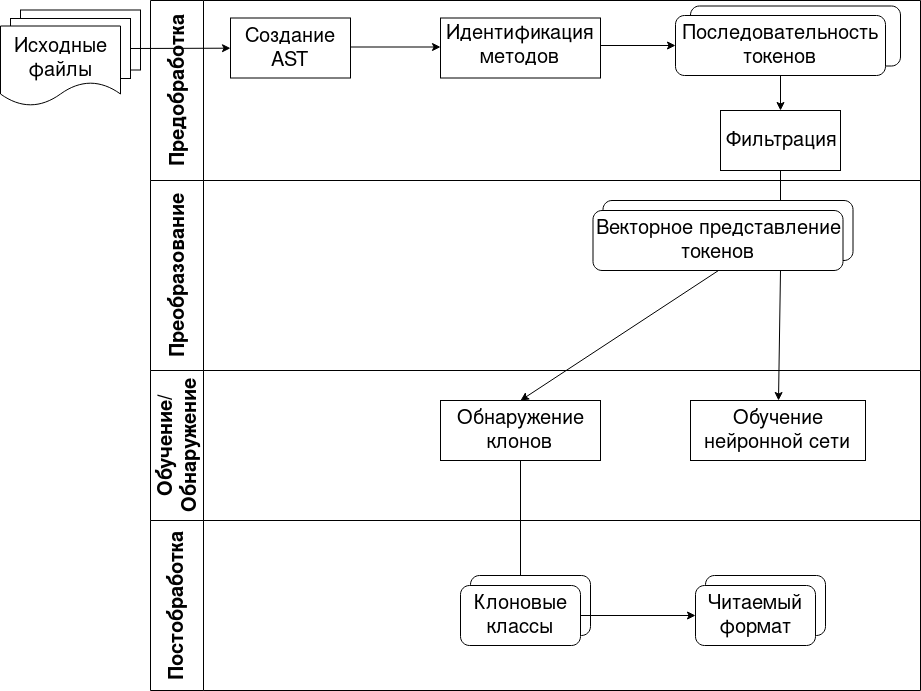
\includegraphics[width=\textwidth]{struct.png}
\caption{Общая структура процесса обнаружения клонов}
\label{fig:struct}
\end{figure}

%%%%%%%%%%%%%%%%%%%%%%%%%%%%%%%%%%%%%%%%%%%%%%%%%%%%%%%%%%%%%%%%%%%%%%%%%%%%%%%%
\section{Предобработка}

На данном этапе, с помощью анализатора, основанного на части среды разработки (IDE Intellij IDEA community), производится представление исходного кода программы в виде AST. После чего, из полученного дерева выделяются только те поддеревья, которые относятся к методам или функциям. Такой поиск осуществляется посредством обхода в глубину всех вершин AST. В случае обнаружения вершины искомого типа, дальнейший спуск в данную ветку не осуществляется.

\nomenclature{IDE}{Integrated Development Environment}

Следующим этапом полученные поддеревья преобразуются в последовательности токенов путем того же обхода в глубину всех их вершин. После чего производится фильтрация этих последовательностей. Производимая фильтрация позволяет исключить влияние незначительных отличий фрагментов исходного кода друг от друга. В рамках данного подхода фильтрации подвергаются токены следующих типов:
\begin{itemize}
\setlength\itemsep{0mm}
\item комментарии различного типа
\item элементы форматирования
\item списки параметров
\end{itemize}

Обычно, для обнаружения клонов выше клонов I типа, необходимо производить анонимизацию токенов. Однако, в нашем методе, нейронная сеть будет сравнивать типы токенов. Из этого можно сделать вывод о ненадобности анонимизации. Таким образом, процесс фильтрации - последний процесс на этапе предобработки.
%%%%%%%%%%%%%%%%%%%%%%%%%%%%%%%%%%%%%%%%%%%%%%%%%%%%%%%%%%%%%%%%%%%%%%%%%%%%%%%%
